\cotefile{83}
\scanpage{46}
\mspage{8}
Autre façon de le dire :

$\rho_{ijkl}$ ne dépend que du
``carré'' $(i,j)(k,l)$ muni d'une section
du produit contracté des \deleted{\illegible{1}}diagonales,
i.e. d'une codiagonale, car
\[
\deleted{\unsure{\mathrm{car}}}\quad
\rho_{(i,j)(k,l)}=\rho_{(k,l)(i,j)}
\tag*{(9)}
\]
\figure{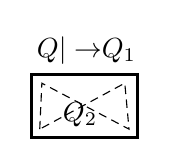
\begin{tikzpicture}[x=1.35cm,y=0.8cm]
\draw[very thick] (0,0) rectangle (1,1);
\draw[densely dashed] (0.08,0.13)--(0.10,0.86)--(0.92,0.13)--(0.88,0.86)--cycle;
\node[above] at (.52,1) {$\deleted{\unsure{Q|\rightarrow}}Q_1$};
\node at (.46,.36) {$Q_2$};
\end{tikzpicture}}
\margin{$Q_3$ est le troisième carré}

(\uline{NB} Cette relation n'a de sens que parce que
$\operatorname{End}(W)$ est supposé commutatif)

On se donne une \deleted{\unsure{carré|coin}} str. carr. ou
codiag. de $I$, $\sim$ se donner
un repère de l'ens $\operatorname{Car}(I)$ des
structures \unsure{carrées|carrés|coin}, et la donnée de
% slanted
\margin{\uline{vérifier la} \uuline{compatibilité}. Il faut peut-\unsure{ê} twister par un (\unsure{aut}) de $\mathfrak S_3$\ldots}
équivaut à une application de
\[
\underbrace{\operatorname{Rep}\operatorname{Car}(I)}_
{\substack{\text{torseur}\\\text{sous }\text{\uuline{$\mathfrak S_3$}}}}
\longrightarrow \unsure{\mathcal U|U}(k)
\]

Il reste à décrire la catégorie des
\unsure{quadrités|quadralités} dans $C$, \deleted{\unsure{la don}} de façon
plus simple que par un système
de $24$ flèches $u_{(i,j)(k,l)}$ deux à deux opposées.
% archive sheet number: 45
\scanpage{48}
\margin{Avril 86}
\uline{Trialités}\qquad Soit $C$ catégorie, $n$ entier naturel $\geq\deleted{\unsure{3}}2$.
\inserted{(le cas $n=2$ trivial)}
On appelle $n$-alité (trialité, quadralité, pentalité si $n=3,4,5$)
un système
\[
\{I,E,\{E_i\}_{i\in I},(\varphi_i)_{(i\in I)}\}
\]
où \quad $I$ \deleted{\unsure{ens|ens.}} de cardinal $n$,
\[
\varphi_i:E\mathrel{\unsure{-|\to}}E_i\qquad i\in I
\]
flèches de $C$, satisfaisant

$\forall J\subset I$ avec $\operatorname{card}J=2$, l'application
\[
E\xrightarrow{\varphi_J}\underbrace{E_J=\prod_{i\in J}E_i}_{
\substack{\deleted{\text{on suppose que}}\\\deleted{\text{ce produit existe,}}\\
\deleted{\forall J\in\unsure{\mathfrak P_2|\mathcal P_2}(I)}}}
\tag*{(1)}
\]
est un \uline{iso} (dans $\widehat C$) $E$ entouré des $\varphi_i$ $(i\in J)$ est un produit des
$E_i$ dans $C$.

\margin{[\, Les $n$-alités forment une catégorie $n$-al$(C)$, fibrée sur le groupoïde \deleted{\unsure{Ens}}\unsure{$\mathcal S_n$|$\mathrm{Ens}_n$}}

Je m'intéresse surtout \deleted{aux} deux cas

$1^\circ)$ $C$ catégorie additive

$2^\circ)$ $C=\mathrm{Ens}$

\deleted{Dans le cas \unsure{2}} Je vais ici, regarder le cas $2^\circ)$

Si un des $E_i$ est vide, alors \inserted{$E$ l'est et} tous sauf au plus
un le sont. On va exclure ce cas, \inserted{dit} ``impropre''.

Dans tous les autres cas les $E_i$ peuvent
être considérés comme des quotients de $E$.
Ainsi, la structure peut être considérée comme
portée par $E$\deleted{\unsure{,}} \inserted{$I$}, \deleted{muni d'une}, une
application $I\mathrel{-}\operatorname{Quot}(E)$. Cette application
est d'ailleurs injective, sauf \deleted{quand \unsure{tous les}}\inserted{dans}
% archive sheet number: 47
\scanpage{49}
le cas où tous les $E_i$ sont réduits à un
élément \deleted{\unsure{et}} ($\Leftrightarrow$ \deleted{\unsure{il}} un des $E_i$ l'est $\Leftrightarrow E$ l'est),
cas dit ``trivial''. Donc une $n$-alité non
triviale peut être considérée comme
un ens $E$ \unsure{munie|muni} d'une partie
$I\subset\operatorname{Quot}(E)$, avec $\operatorname{Card} I=n$, et \unsure{ou|un|satisfaisant}
l'axiome évident traduisant (1).

Autre version : Soit \deleted{\unsure{$S$}}
\[
S=\coprod_{i\in I}E_i\qquad\text{(``sommets'')}
\tag*{(2)}
\]
et \deleted{\unsure{$f$}} soit
\[
R\subset S\times E \tag*{(3)}
\]
défini par
\[
(\underset{\substack{\Vert\\(i\in I,s_i\in E_i)}}{s},
 \underset{\substack{\uparrow\\E}}{x})\in R\quad\Longleftrightarrow\quad
s=\varphi_i(x)
\]

\deleted{Alors on a ceci}

Considérons
\[
E\longrightarrow \unsure{\mathcal P|P|\mathfrak P}(S)\qquad x\longmapsto R(\unsure{a|x})\subset\deleted{E}S
\]
les éléments de \deleted{$R(x)$} la forme $R(x)$ sont
appelés $n$-uples de $S$. On dit que
\deleted{\unsure{a)} $E\longrightarrow\mathcal P(S)$ est \unsure{+}}
$a\in\mathcal P_2(S)$ est une \uline{arête} si \unsure{$a$|\deleted{$a$}|elle} est \unsure{contenu|contenue}
dans un $n$-uple, i.e. $\{s,t\}$ est une arête
sss $s\ne t$ et $\exists x\in E$ tel que $\{s,t\}\subset R(x)$ i.e.
% archive sheet number: 48
\scanpage{50}
$(s,x),(t,x)\in R$. On a

(i) $\forall s,t\in S\quad s\ne t$, existe au plus un $\unsure{a|x}\in E$
tel que $(s,x),(t,x)\in R$ i.e. $s,t\in R(x)$ i.e.
$\{s,t\}\subset R(x)$

\margin{\deleted{[\uline{NB} Cette condition est symétrique en $S,R$ elle signifie en fait \unsure{soit|si $s\ne t$} $x\ne y$ $(s,t\in S,\ x,y\in R)$ alors il existe au moins un $\{s,t\}$ \unsure{$s\mapsto x$}}}
\deleted{(ii) La relation dans $S$ :}

\uline{NB} Cette \deleted{relation}\inserted{condition} est symétrique en $S,R$. Elle
signifie que si $a\in\unsure{\mathcal P|P|\mathfrak P}_2(S)$, $u\in\mathcal P_2(R)$,
alors $\exists s\in a,\ \unsure{a|x}\in u$ tels que $\deleted{\unsure{R}}(s,x)\notin R$
% slanted
\margin{toute arête contenue dans \unsure{exactt} un $n$-uple}

Si on suppose que les \deleted{$R(x)$} $\operatorname{card}R(x)\geq2$
\deleted{\illegible{1}}\deleted{\unsure{alors}} (ce qui est le cas quand ça provient
d'une \deleted{\unsure{tri}} $n$-alité, \deleted{(cas \unsure{impropre})}\inserted{auquel cas $\operatorname{card}R(\unsure{n|x})=\deleted{\unsure{S}}n$}), alors
$R\longrightarrow\mathcal P(S)$ est injectif. De $=$, si on
suppose que pour tt $s\in S$, $ {}^{s}\!R(s)\subset R$ est
de cardinal $\geq2$ (ce qui est le cas si
ça provient d'une $n$-alité propre non triviale)
alors $S\longrightarrow\mathcal P(R)$ injectif)

(\unsure{ii|vi}) La relation dans $S$
\[
\{s,t\}\text{ n'est pas une arête}
\]
(i.e $s=t$ ou $\deleted{\unsure{\in|\nexists}}\nexists x\in E$ tel que $\{s,t\}\unsure{\subset|\not\subset}R(x)$)
est une relation d'équivalence dans $S$
i.e. pour \unsure{toute|une} arête $\{\unsure{r|s},t\}$, tout
sommet de $S$ est \unsure{liée|lié} soit à $r$, soit
à $t$.

Cette condition (ii) implique que $S=\coprod E_i$
de telle façon que \inserted{pour} $a\in\mathcal P_2(\unsure{R|S})$, $a$ est une
% archive sheet number: 49
\scanpage{51}
arête sss $a$ n'est contenu dans aucun
des $S_i$. D'autre part, si $u$\inserted{$\subset S$} est un
$n$-uple, alors
\[
u\longrightarrow I
\]
est injectif \inserted{(i.e. $u\cap E_i$ de card $\leq1$ pour tt $i$).} Dire que c'est aussi surjectif
(ce qui est vérifié dans le cas d'une $n$-alité)
signifie ceci

(iii) $\forall s\in S,\ x\in R$, existe $s'\in S$ tel que
$\{s,s'\}$ ne soit pas une arête (p.ex. $s'=s$) et $(s',x)\in R$
(NB en vertu de (ii) cet $s'$ est unique).
% slanted
\margin{implique que tous les $R(x)$ sont de $=$ cardinal $n=\operatorname{card}I$}

Alors on a
\[
\varphi_i:E\longrightarrow\deleted{\unsure{S_i}}E_i
\]
en associant à tout $x\in E$ \deleted{le système}
\deleted{des} $\varphi_i(x)\in E_i$ tel que $\{\varphi_i(x)\}=S(x)\cap E_i$

(iv) \deleted{\unsure{$\exists s,s'$} \illegible{1}} $\exists x\in E$ tel que $R(x)$ de card $\geq2$.
\[
(\Longleftrightarrow\operatorname{card}I\geq2)
\]

\uline{NB} Dans le cas contraire, tous les $R(x)$
sont de cardinal $1$ (On suppose $S\ne\unsure{0|\varnothing}$)
et $R$ est le graphe d'une
application $E\mathrel{\unsure{-|\to}}S$

\begin{center}\rule{1.2cm}{.6pt}\end{center}
% archive sheet number: 50
\scanpage{52}
% sheet: cover
Biicosaèdre et cartes
de congruence

avril 1986
% archive sheet number: 51
\scanpage{53}
\margin{Avril 86}
\uline{Biicosaèdre \inserted{\uline{pas} \uline{\unsure{gauche|gauches}} \uline{et}} orientations}

Soit $(S,\{\deleted{\unsure{\Phi,\Phi'|\mathcal I,\mathcal I'}}\})$ un biicosaèdre \inserted{gauche} orienté, et soit
$\widetilde S_\Phi,\widetilde A_\Phi,\widetilde F_\Phi$ le revêtement \deleted{des} orienté de $(S,\Phi)$
$\widetilde S_{\Phi'},\widetilde A_{\Phi'},\widetilde F_{\Phi'}$ celui de $(S,\Phi')$.
\inserted{Ce sont des icos. ``droits'' orientés.} On va définir des
bijections
\[
\begin{aligned}
\varepsilon^S_{\Phi',\Phi\deleted{\unsure{'}}}&:\widetilde S_\Phi\mathrel{\overset{\sim}{\longrightarrow}}\deleted{\widetilde A}\widetilde S_{\Phi'}\\
\varepsilon^A_{\Phi',\Phi\deleted{\unsure{'}}}&:\widetilde A_\Phi\mathrel{\overset{\sim}{\longrightarrow}}\deleted{\unsure{\widetilde S}}\widetilde A_{\Phi'}\\
\varepsilon^F_{\Phi',\Phi\deleted{\unsure{'}}}&:\widetilde F_\Phi\mathrel{\overset{\sim}{\longrightarrow}}\widetilde F_{\Phi'}
\end{aligned}
\]
\margin{(voir rectification, il faut remplacer $\widetilde A_\Phi,\widetilde A_{\Phi'}$ par $\overline A_\Phi$ et $\overline A_{\Phi'}$, ens des arêtes \uline{orientées})}
comme voici.

\deleted{\unsure{$\widetilde S_\Phi$}} La fibre de $\widetilde S_\Phi$ et $\widetilde S_{\Phi'}$ en un point $s\in S$ sont les
deux \inserted{\deleted{\unsure{deux}} ens. des orientations des deux} structures pentagonales sur $S\smallsetminus\{s\}$ associées
\deleted{de} l'une à $\Phi$, l'autre à $\Phi'$, et qui sont associées. \deleted{Elles}
ont $=$ groupe des rotations, \inserted{$U_s$}, \deleted{\unsure{isomorphe}} qui
est un \deleted{espace aff.} $\mathbb F_5$-module libre de rang $1$,
et $U_s^*$ (ens des générateurs) est un torseur sous le groupe cyclique
$\mathbb F_5^*$ \inserted{iso à $\mathbb Z/4\mathbb Z$}, \deleted{\unsure{leurs}}
\deleted{par \illegible{2} l'élément $2$}
\margin{On voit $U_s^*$ \unsure{s'identifiant|distinguer} \unsure{longueur} de}
\figure{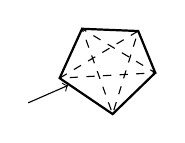
\begin{tikzpicture}[scale=.57]
\coordinate (a) at (0,.1);\coordinate (b) at (.5,1.2);\coordinate (c) at (1.75,1.15);\coordinate (d) at (2.13,.22);\coordinate (e) at (1.18,-.70);
\draw[thick] (a)--(b)--(c)--(d)--(e)--cycle;
\draw[dashed] (a)--(c)--(e)--(b)--(d)--cycle;
\draw[->] (-.7,-.45)--(.19,-.06);
\end{tikzpicture}}
% slanted: note beside the pentagon
$(\widetilde S_\Phi)_s$ est l'une des classes modulo le sous-groupe $\pm1$
soit $\{u,-u\}$, et $\widetilde S_{\Phi',s}$ est l'autre classe, donc
$\{2u,\deleted{\unsure{u}}-2u\}$.

L'application
\[
\varepsilon^S_{\Phi,\Phi'}(s):\widetilde S_\Phi(s)\longrightarrow\widetilde S_{\Phi'}(s)
\quad\text{est donnée par}\quad
u\longmapsto 2u
\]
On aura
\[
\deleted{\unsure{\varepsilon}}\varepsilon_{\Phi',\Phi\deleted{\unsure{'}}}(s)
\deleted{\unsure{\varepsilon}}\varepsilon^{\deleted{\unsure{2a|S}}}_{\Phi,\Phi'}(s)
=\deleted{\unsure{a}}u\longmapsto4u=-u=\underline a_{\Phi'}u
\]
($\underline a_{\Phi'}$ l'antipodisme de $\Phi'$,
et de $=$ en sens inverse. (Si on avait choisi
$u\mapsto3u$\inserted{$=-2u$}, ça aurait été pareil, car
$\inserted{3^2=(-2)^2}\deleted{\unsure{4}}\equiv-1\ (5)$)
\deleted{\unsure{tout comme} $4\equiv-1\ (5)$)} Donc
% slanted
\margin{On a \unsure{l'iso} can (indépendt du choix de $\Phi$ dans $\{\Phi,\Phi'\}$) $\widetilde S_{\Phi(s)}\unsure{\times|\wedge}\widetilde S_{\Phi'}(s)\simeq\{\Phi,\Phi'\}$ les deux choix différant par $\underline a_\Phi$ (ou $\underline a_{\Phi'}$) \deleted{On voit \unsure{ainsi}}}
\[
\left\{\begin{aligned}
\varepsilon_{\Phi',\Phi}\varepsilon_{\Phi,\Phi'}&=a_{\Phi'}\qquad\text{et de }=\\
\varepsilon_{\Phi,\Phi'}\varepsilon_{\Phi',\Phi}&=a_\Phi
\end{aligned}\right.
\tag*{(1)}
\]
\margin{donc l'identification entre $\widetilde S_\Phi$ et $\widetilde S_{\Phi'}$ dépend du choix d'un $\Phi$ ou de $\Phi'$, dans $\{\Phi,\Phi'\}$}

Soit une face $t$ de $\Phi$, $t'$ sa complémentaire, face de $\Phi'$.
on a une bijection canonique
\[
\alpha^{\deleted{\unsure{S}}}_{\Phi',\Phi}:\unsure{t'_\Phi|t_\Phi}\simeq t_{\Phi'}\quad \deleted{\unsure{t}}\quad
\text{(et $\alpha_{\Phi,\Phi'}$ est l'inverse !)}
\]
d'où
\[
\varepsilon^F_{\Phi',\Phi}:
\underset{\substack{\Vert\\\widetilde A_{\Phi,t}}}{\omega(t_\Phi)}
\xrightarrow{\sim}\underset{\substack{\Vert\\\widetilde A_{\Phi',t'}}}{\omega(t_{\Phi'})}
\]
% archive sheet number: 52
\scanpage{54}
d'où $\varepsilon^F_{\Phi',\Phi}$. Cette fois on aura
\[
\left\{\begin{aligned}
\varepsilon^{\deleted{\unsure{S}}F}_{\Phi',\Phi}\circ\varepsilon^F_{\Phi,\Phi'}&=\mathrm{id}_{F_{\Phi'}}\qquad\text{et de }=\\
\varepsilon^F_{\Phi,\Phi'}\circ\varepsilon^F_{\Phi',\Phi}&=\mathrm{id}_{F_\Phi}
\end{aligned}\right.
\]

Soit enfin $a$ une arête commune à $\Phi,\Phi'$
i.e. $a\in\unsure{\mathcal P|P|\mathfrak P}_2(S)$. Alors $S\smallsetminus\{a\}=\alpha_\Phi\amalg\alpha_{\Phi'}$, où $\alpha_\Phi$ est
formé des deux éléments \inserted{$u$}\deleted{\unsure{$s$}} de $S\smallsetminus\{a\}$ tels que
$(S\smallsetminus\{a\})\cup\{u\}\in\Phi$, et \unsure{item|idem|itou} pour $\alpha_{\Phi'}$. On a bij. can.
\figure{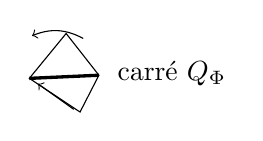
\begin{tikzpicture}[scale=.57]
\draw (0,.1)--(.82,1.1)--(1.55,.17)--(1.13,-.65)--cycle;
\draw[very thick] (0,.1)--(1.55,.17);
\draw[->] (1.2,.99) to[bend right=25] (.06,1.05);
\draw[->] (.99,-.59)--(.19,-.02);
\node[right] at (1.75,.2) {carré $Q_\Phi$};
\end{tikzpicture}}
\[
\begin{aligned}
\widetilde A_{\Phi,a}&\simeq a\wedge\alpha_\Phi\quad\inserted{(\simeq\omega(Q_\Phi))}\qquad\text{et de }=\\
\widetilde A_{\Phi',a}&\simeq a\wedge\alpha_{\Phi'}
\end{aligned}
\]
donc
\[
\widetilde A_{\Phi,a}\wedge\widetilde A_{\Phi',a}\simeq\alpha_\Phi\wedge\alpha_{\Phi'}\simeq a
\]
\margin{(NB on a $a\wedge a_\Phi\wedge a_{\Phi'}\overset{\mathrm{can}}{=}1$ à cause de l'orientation canonique de l'ens $S$ comme de $\{\Phi,\Phi'\}$).}

Donc choisir une bijection entre $\widetilde A_{\Phi,a}$ et $\widetilde A_{\Phi',a}$, \deleted{\unsure{revient}}
à choisir un élément de $a$, \inserted{i.e. une orientation de l'arête $a$}.
Donc on n'a pas
vraiment ici de bijection canonique au niveau
de $\widetilde A_\Phi$ et $\widetilde A_{\Phi'}$ comme annoncé. Ainsi, on
trouve une bijection
\[
\deleted{\unsure{\varepsilon}}\varepsilon^{\vec A}_{\Phi',\Phi}:
\overrightarrow{\widetilde A}_\Phi\xrightarrow{\sim}\overrightarrow{\widetilde A}_{\Phi'}
\qquad\text{et de $=$ en sens inv.}
\]
satisfaisant cette fois
\[
\left\{\begin{aligned}
\varepsilon^{\vec A}_{\Phi',\Phi}\,\varepsilon^{\vec A}_{\Phi,\Phi'}&=\mathrm{id}_{\overrightarrow{\widetilde A}_{\Phi'}}\qquad\text{et de }=\\
\varepsilon^{\vec A}_{\Phi,\Phi'}\,\varepsilon^{\vec A}_{\Phi',\Phi}&=\mathrm{id}_{\overrightarrow{\widetilde A}_\Phi}
\end{aligned}\right.
\]
% slanted
\margin{\uline{NB} $\overrightarrow{\widetilde A}_\Phi\simeq\operatorname{Rep}^{+}\deleted{\unsure{\Phi}}\inserted{(S,A,\Phi)}$, $\overrightarrow{\widetilde A}_{\Phi'}\simeq\operatorname{Rep}^{+}\inserted{(S,A,\Phi')}$}

En résumé : Pour les dodécaèdres \deleted{\unsure{duaux|des}}\inserted{$D,D'$} duaux
des icosaèdres $\widetilde{(S,A,\Phi)}=I$ et $\widetilde{(S,A,\Phi')}=I'$, \deleted{il y a}\inserted{on}
peut considérer $D,D'$ \unsure{pointés|portés|précisés} par \uline{le $=$} ens
de sommets (le choix de l'identification \unsure{en|ne}
dépendant \unsure{pas|par} du choix d'un $\Phi\in\{\Phi,\Phi'\}$),
mais l'analogue au niveau $I,I'$ n'est
pas vrai : le choix d'une identification des
sommets . $S(I)\simeq S(I')$ dépend du choix de $I$ ou $I'$.
% archive sheet number: 53
\scanpage{55}
et est remplacé par son produit par l'antipodisme
(à droite, ou à gauche, c'est kif kif) si on remplace
$\Phi$ par $\Phi'$.

On appellera \uline{biicosaèdre orienté} une \deleted{système}
\deleted{famille à deux éléments $\{I,I'\}$ de \unsure{la une}}
\deleted{\unsure{str|de}} un polyèdre comb. orienté avec
deux comp. connexes $I,I'$, qui sont
des icosaèdres, et la donnée d'un ens. \inserted{$\{\theta,\theta'\}$}
de \uline{deux} bijections \inserted{(= correspondances)} entre $S(\deleted{\unsure{J}}I)$ et $S(I')$
\deleted{\unsure{chacun de la|classe de}}
commutant aux antipodismes, et
\deleted{\unsure{formant}} tel que $\theta'$ et $\theta$ sont \unsure{déduits|déduites|déduisent} l'un de
l'autre par comp. avec l'antipodisme,
et tel que, en passant au quotient \deleted{\unsure{sous}}\inserted{de $\theta$}
\unsure{et|ou} $\theta'$ modulo antipodisme, la
bijection qu'on obtient entre $S(I)/\underline a$ et $S(I')/\underline a$
\deleted{transforme la bijection de \unsure{icos|l'icos}}
donne sur l'ens commun deux structures
d'icosaèdres gauches \deleted{\unsure{opp}} complémentaires!
% slanted
\margin{et les bijections, \unsure{antér.ieures|antérieurement|extérieures} soient définies \unsure{resp}$^t$ par $\varepsilon^S_{\Phi,\Phi'}$ et $\varepsilon^S_{\Phi',\Phi}$}

Il revient au $=$ de dire que l'on se donne
\deleted{une donnée d'ident. antérieure des}
\deleted{$I'$ avec l'icos. complémentaire à}
\inserted{une paire d'iso orientés}
\[
\left\{\begin{aligned}
\overline I'&\xrightarrow[\sim]{\alpha_{I'}}\operatorname{compl}.(\overline I)\\
\overline I&\xrightarrow[\sim]{\alpha_I}\operatorname{compl}(\overline I')
\end{aligned}\right.
\]
\margin{icos. ``complémentaire'' à $\overline I$, avec l'orientation canonique déduite}
dont les composés soient les antipodismes
\[
\unsure{\alpha_I}\ \operatorname{compl}(\alpha_{I'})\alpha_I:
I\mathrel{\unsure{-|\to}}\underbrace{\operatorname{compl}\operatorname{compl}(I)}_{
\substack{\Vert\\-I,\ \text{i.e. }I\\\text{avec l'orientation}\\\text{opposée}}}
\]
soit l'antipodisme, qui est un
iso de $I$ avec $-I$
% archive sheet number: 54
\scanpage{56}
Si on a deux biicosaèdres orientés
$\{I_1,I'_1\}$ et $\{I_2,I'_2\}$, le choix d'une \deleted{icos. orient}
composante connexe du premier, et d'un
iso de celle-ci avec une comp. conn. de
l'autre, se prolonge de façon unique en
un isom des biicosaèdres orientés.

La paire \deleted{\unsure{$I$}} $(\widetilde I_\Phi,\widetilde I_{\Phi'})$ des rev. orientés
des deux struct. icosaèdrales \inserted{gauches} complémentaires,
est un biicos. orienté, et son groupe des
autom est celui du \deleted{groupe} biicosaèdre
gauche de départ.

Une autre façon de dire les choses est
celle-ci. Considérons un biicosaèdre droit
non orienté $I$. On lui associe l'icosa
complémentaire $I^{\unsure{\circ|o}}$, tel que pour $s,s'\in S=S(I)$
$\{s,s'\}$ soit arête de $I^\circ$ sss $\{s,\underline a(s')\}$ est arête de
$I$ (où $\underline a$ est l'antipodisme). On a donc
$I=I^{\circ\circ}$. \deleted{\unsure{On} le groupe des} Une structure
de biicosaèdre sur $S$ (\deleted{\unsure{sur|ensemble}} de douze sommets
est une paire de structures icosaédrales
$\{I,I'\}$ sur $S$, mutuellement complémentaires.

Le groupe des autom s'envoie dans
le groupe aux \inserted{(\unsure{sur}) le groupe des} permutations de $\{I,I'\}$, donc
\[
1\longrightarrow
\underset{\substack{\simeq\operatorname{Aut}(I')\\
\simeq\operatorname{Aut}^{+}(I)\times\pm1\\
\simeq\operatorname{Aut}^{+}(I')\times\pm1}}{\operatorname{Aut}(I)}
\longrightarrow\operatorname{Aut}(I,I')\longrightarrow\mathbb Z/2\mathbb Z
\longrightarrow\unsure{1|0}
\]
% archive sheet number: 55
\scanpage{57}
Le groupe quotient
\[
\operatorname{Aut}(I,I')/
\underbrace{\operatorname{Aut}^{\unsure{0+|o+}}(I,I')}_{
\substack{\text{autom. qui}\\\text{respectent }I,I'\\\text{et l'orientation}\\
\text{de }I,\ \text{i.e. de }I'}}
\]
est isomorphe à \uline{$\mathbb Z/4\mathbb Z$} sauf erreur.
Mais si on \deleted{\unsure{est|veut}} se donne une
\deleted{\unsure{comme}} \deleted{\unsure{str} biicosaèdre orienté}
orientation de $I$ et une de $I'$ (pour
définir une notion de biicosaèdre \uline{orienté})
\deleted{on \unsure{trouve}}\inserted{d'où} $\unsure{\vec I|\overline I}$ et $\vec I'$, cela nous permet
de choisir \unsure{l'un|\deleted{un}} des icos. de la structure
biicosaédrale de façon canonique -- \unsure{nommément|comme}
celui pour lequel l'orientation de l'autre
soit ``associée''. Donc on ne trouve pas
la bonne notion !

Par contre, il y a un groupe $\mathbb Z/4\mathbb Z$
qui opère sur la catégorie des
icosaèdres orientés, dont le générateur est
\deleted{le passage de} est le passage de $\vec I$ à $\vec I^\circ$.
Le carré du générateur est le passage
de $I$ à $-I$ -- correspond à l'ext.
triviale de $\mathbb Z/2\mathbb Z\subset\mathbb Z/4\mathbb Z$ par
$\operatorname{Aut}(\vec I)^+$, savoir le groupe des autom
de \deleted{Aut} $I$ (ne respectant pas l'orientation)
% archive sheet number: 56
\scanpage{58}
Ainsi, il y a deux extensions, à ne pas
confondre, ayant comme noyau le
groupe de l'icosaèdre orienté
\[
\begin{aligned}
0\longrightarrow\operatorname{Aut}(\vec I)&\longrightarrow
 \operatorname{Aut}(\underbrace{\{\vec I,\vec I^{\unsure{\circ|o}}\}}_{\text{bicos. or.}})
 \mathrel{\unsure{-|\to}}\mathbb Z/2\mathbb Z\longrightarrow0\\
0\longrightarrow\operatorname{Aut}(\vec I)&\mathrel{-}
 \operatorname{Aut}(\{I,I^\circ\})\longrightarrow\mathbb Z/4\mathbb Z\longrightarrow0
\end{aligned}
\]

Il n'y a pas, je crois, d'hom \unsure{dans|de} un sens
ou de l'autre, induisant l'identité
sur $\operatorname{Aut}(\vec I)$. De haut en bas, le gén. de
$\mathbb Z/2\mathbb Z$ (qui définit l'autom ext. non trivial
de $\operatorname{Aut}(\vec I)$) devrait aller sur l'un des
deux gén. de $\mathbb Z/4\mathbb Z$, impossible !

Dans l'autre sens, un \deleted{\unsure{autom}.} $\mathbb Z/4\mathbb Z\longrightarrow\mathbb Z/2\mathbb Z$
doit être surjectif ($=$ \unsure{raison|raison.|va}) le noyau
\deleted{\unsure{doit être|devrait}} de $\operatorname{Aut}(I,I^{\prime})$ est un sous-groupe
d'ordre $2$ -- l'antipodisme ! Et en fait,
je vois maintenant que $\operatorname{Aut}(\vec I,\vec I^{\unsure{\prime|\circ}})$ est \inserted{iso}
\deleted{le quotient} au quotient de \deleted{\unsure{par}} $\operatorname{Aut}(I,I')$
par l'antipodisme. Mais cela semblerait
indiquer qu'il y aurait un foncteur
\[
\text{biicosaèdres (droits) non orienté}\longmapsto\substack{\text{biicosaèdre}\\\text{orienté}}
\]
et en effet, on passe par biicosaèdres
gauches, et biicosaèdres orientés via rev.
des orientations.
% archive sheet number: 57
\scanpage{59}
La théorie générale des cartes de congruences
nous donne
\[
1\mathrel{\unsure{-|\to}}\underbrace{\mathrm{Sl}(2,\mathbb F_5)/{\pm1}}_{\operatorname{Aut}(\vec I)}
\longrightarrow\mathrm{Gl}(2,\mathbb F_5)/{\pm1}
\longrightarrow\underset{\substack{\wr\Vert\\\mathbb Z/4\mathbb Z\quad!!!}}{\mathbb F_5^*}\longrightarrow1
\]

Le groupe $\mathrm{Gl}(2,\mathbb F_5)$ permute entre elles
\unsure{l'ens|l'une} des $4$ structures d'icos. orienté
portées par l'ens $S$ à $12$ éléments, et
ce via le groupe cyclique $\mathbb Z/4\mathbb Z$.

\begin{center}\rule{1.5cm}{.6pt}\end{center}

On doit pouvoir plonger les deux extensions
(de $\mathbb Z/4\mathbb Z$, et de $\mathbb Z/2\mathbb Z$) par $\operatorname{Aut}^+(\deleted{\unsure{\vec I}}I^{\unsure{\circ|o}})$, dans le
groupe produit \deleted{\unsure{$\operatorname{Aut}(I)$}}
$\underbrace{\unsure{\mathrm{GP}|\mathrm{G}\Phi|\mathrm{PGl}}(1,\mathbb F_5)}_{\simeq\mathfrak S_5,\ \text{ordre }120}\times\mathbb F_5^*$, en
l'occurrence (et canoniquement) dans
\deleted{\unsure{donc}} $G=\operatorname{Aut}(I)\times\underbrace{\mathbb F_5^*}_{\simeq\mathbb Z/4\mathbb Z}$.
\unsure{Ce|Cela} groupe est
réalisé comme un groupe d'automorphismes
de \deleted{\unsure{ce}} \deleted{\unsure{quadriicosaèdre|bi-icosaèdre}}\deleted{polyèdre}\inserted{\unsure{des cartes|double|doubles}}
$I\amalg I'$, mais en
respectant la structure supplémentaire
donnée par un iso $I/\mathrm{antip.}\simeq I'/\mathrm{antipod.}$\inserted{($\simeq J$ ic. g.)}

Choisissant une orientation sur $I$, une autre
sur $I'$ (ce qui permet d'identifier $\vec I,\vec I'$ l'un
et l'autre au rev. \deleted{universel}\inserted{orienté} de $J$) on trouve
% slanted
\margin{\uline{NB} Ce sous-groupe est indép. du choix des orientations : \unsure{il est} \deleted{\unsure{précisément}}\inserted{donné par}}
un sous-groupe respectant ces orientations
$\deleted{\unsure{\mathrm A}}\operatorname{Aut}^{+}(I)=\operatorname{Aut}^{+}(\vec I)$. Le quotient \inserted{(d'ordre $8$)} opère
sur l'ens des quatre orientations de $(I,I')$, et \deleted{les}
% archive sheet number: 58
\scanpage{60}
c'est le groupe des autom du carré combinatoire
\deleted{\unsure{permutant|permute} entre elles de} qu'elles forment
\inserted{($\simeq\mathfrak S_{5}$)}, \deleted{\unsure{qui} se forment
\unsure{orientations}}. L'ext. de $\mathbb Z/2\mathbb Z$ par $\operatorname{Aut}^+(I)$
est l'image inverse du sous-groupe \unsure{d'|de}
ordre 2 \inserted{(qui fixe \unsure{le|les} \deleted{deux} \unsure{côté|côtés} du carré correspondant
aux choix des deux orientations (mais qui peuvent échanger ses deux extrémités).}
\deleted{\unsure{partie du cr} \unsure{\illegible{2}|de l'antipodisme} de carré}
\deleted{de $\{\pm1\}$ de $\mathbb F_5^*$, c'est le groupe
des autom du système, respectant la
paire d'orientations (sans nec$^t$ fixer
la comp. conn. corresp.). L'ext.}
L'ext. de $\mathbb Z/4\mathbb Z$ par $\operatorname{Aut}^+(I)$ s'obtient en prenant
l'image inverse du groupe des rotations
du carré. L'intersection de ces deux
sous-groupes de $G$ est $\operatorname{Aut}^+(I)$
(\unsure{se projette} dans le groupe des autom du
carré). \deleted{\unsure{L'é}}Le groupe engendré est formé
des produits, et c'est $G$ tout entier \ldots

\uuline{Généralisation} aux cartes de congruences.

La carte $\unsure{\mathrm{Cong}|\mathrm{Congr}}_{n}$ étant réalisée avec \deleted{des}\inserted{l'ens des sommets $S$ formé}
\deleted{sommets qui sont des} paires $\{a,-a\}$
d'éléments d'un $\mathbb Z/n\mathbb Z$-module libre \inserted{symplectique $E$} de
rang $2$, formant base, on peut y
% slanted
\margin{Supposer $n$ premier i.e. $\mathbb Z/n\mathbb Z$ un corps, ici ??}
associer $a\otimes a\in\operatorname{End}(E)=M$, \inserted{(alg. Az.)} ce sont
des éléments du cône isotrope $C$ de $M^{\unsure{\natural|\sharp|0}}_{\unsure{s|8}}$
(éléments de trace nulle) \unsure{i.e.|ipso} \unsure{a priori|donc ici|formé} des
nilpotents. On trouve ainsi une réalisation
% archive sheet number: 59
\scanpage{61}
(compatible avec les op. du groupe
$G_n=\deleted{\unsure{\mathrm{Sl}(2,|\mathrm{Sl}(2,\mathbb Z)}}\mathrm{Sl}(E)/{\pm1}$, mais pas du groupe
$\mathrm{Gl}(E)$ tout entier) de $S$ dans ledit cône.

On ne trouve pas tous les éléments non dégénérés
dudit cône, mais \inserted{sur chaque rayon} seulement \deleted{\unsure{tous}} une
classe \deleted{\unsure{en}}\inserted{mod} $\mathbb F_p^*/\mathbb F_p^{\unsure{\times2|*2}}$. Les opérations \inserted{$T_\lambda\ (\lambda\in\mathbb F_p^\times)$} de
$\mathbb F_p^\times=\mathbb Z/n\mathbb Z^*$ sur $S$, sont transformées en
les opérations d'homothétie par les \uuline{$\lambda^2$}.

Mais les homothéties par les $\lambda\in\mathbb F_p^*\smallsetminus F_p^{\times2}$
échangent entre elles les deux
composantes naturelles de l'ens des \deleted{pts}
\inserted{él.} non \deleted{dégénérés}\inserted{nuls} du cône (cette division
en classes, \deleted{indexées par $k$} l'ens des
classes formant un torseur sous $k^\times/k^{\times2}$,
a un sens pour \unsure{tte|les|tt} Alg. d'Azumaya
de rang $4$ sur un corps quelconque $k$ --
si $k$ est fini, \deleted{\unsure{$q/\mathbb F_p$|$\mathbb F_q$}}, de car $\ne2$, $k^\times\deleted{\unsure{/k|/k^\times|/k^{*2}}}$
cyclique d'ordre pair, $k^\times/k^{\times2}$ est d'ordre $2$
\ldots ) Ainsi on trouve une ``bi-structure'',
avec opération de $\unsure{\mathrm{Gp}|\mathrm{GP}|\mathrm{Gl}}(E)\times\mathbb F_p^*$ dessus\ldots.

\hfill TSVP
% archive sheet number: 60
\scanpage{62}
Soit $M$ alg. d'Azumaya sur corps $\mathbb F_p$, $p$ premier impair, et $C^*$ l'ens des éléments nilpotents non nuls de $M$.

Alors \deleted{\unsure{nous}} $C^{\unsure{\times|*}}$ se divise naturellement en deux classes $C_i^*$, \deleted{la multiplication}
\[
\lambda\unsure{\varepsilon|\in} C_i^{\unsure{\times|*}}=C_i^*\quad\mathrm{sss}\quad\lambda\in\underset{\substack{\wr\Vert\\ k^\times/\pm1}}{k^{\times2}}\qquad(\text{pour }\lambda\in k^\times).
\]
\margin{Il y a un seul élément par classe si $p=3$, \unsure{formée|formé} de trois éléments -- ce qui n'est pas bien intéressant !} % slanted

\inserted{Sur $C_i^*$, il y a une str. can. de bi-cartes \uline{orientées} de type \unsure{bipi-Cong|bi-Cong|bi-cartes},} \deleted{Sur chaque $C_i$, il y a une structure de carte orientée canonique, \unsure{de bi-Cong|des bi-cartes}, \unsure{multicarte|multi-cartes}}, et les opérations $\unsure{\overline t_\lambda|t_\lambda|\overline T_\lambda}$, $\lambda\in k^\times/\pm1$, sont les homothéties $\lambda^2$. Le groupe $G\!P_M$\deleted{(\unsure{$\mathbb F_p$})} $\simeq M^\times/k^\times$ \deleted{est \unsure{un|une} \unsure{opérant}} \deleted{sur $C_i$ est le groupe des} groupe des autom des cartes bi-cartes \uline{orientées}, il a un sous groupe d'indice 2 : les autom qui fixent les deux comp. connexes. \deleted{Le groupe $G\!P_M\times k^\times$ est le groupe des autom}

Considérons sur chaque $C_i$ l'ens $\unsure{\mathcal E|E}_i$ : \deleted{qui respectent} des structures de cartes de type \unsure{Cong|$c_i$}, \unsure{déduites|déduire} de la can. $c_i$ par les opérations $T_\lambda$ \uline{par transport de structures}. \inserted{(ce sont donc les $\unsure{\mathcal F|\mathcal E|\overline T}_{\lambda^2}(c_i)$)} (\deleted{\unsure{alors}} Alors, $\{a,b\}$ est une arête pour $T_\lambda(c_i)$ sss \deleted{\unsure{$\mathcal E$}} $\{T_\lambda a,T_\lambda b\}$ \deleted{\unsure{de|dans}} est une pour $c_i$, \uline{et non pas} si $\{a,T_\lambda b\}$ en est une. \deleted{\unsure{Si|de} $\lambda^2$ est l'\unsure{opp.}} Si $\lambda^2=-1$, on trouve donc $T_\lambda(c_i)=c_i$, mais $T_\lambda$ est un autom
% archive sheet number: 61
